\documentclass[11pt,a4paper]{article}

\usepackage[T1]{fontenc}
\usepackage[utf8]{inputenc}
\usepackage[margin=22mm]{geometry}
\usepackage{microtype}
\usepackage{amsmath,amssymb}
\usepackage{booktabs}
\usepackage{graphicx}
\usepackage{xcolor}
\usepackage{subcaption}
\usepackage[hidelinks,breaklinks=true]{hyperref}

\definecolor{ink}{HTML}{14181A}
\definecolor{slate}{HTML}{5C726D}
\definecolor{gold}{HTML}{E6BB58}
\definecolor{paperbg}{HTML}{FBFBF8}

\title{\textbf{Four G Variations}\\[2pt]
\large Semantic Variants of the GraphFin Hero Object}
\author{GraphFin Engineering}
\date{Companion to \emph{From Letterform to Loop}, v1.0}

\begin{document}
\color{ink}
\pagecolor{paperbg}

\begin{abstract}
\noindent
The parent study ranks eight candidate shapes and recommends a single winner.
This note does the opposite and stays inside the brand: it keeps the letter G
and asks what the ring can be made to \emph{mean}. Four variants are rendered
with the production material, lighting, and 40\,degree camera, and each is
justified by a single geometric device that carries a single semantic channel.
Every device is a change to the parameterisation, not to the artwork, so each
variant remains a function rather than a mesh.
\end{abstract}

\section{Design rule}

\noindent
Each variant must satisfy three constraints: it must be a closed or
layer-stacked surface so that the object reads as solid rather than torn; it
must be expressible with the existing two instanced primitive types and one
recycled seam; and it must carry its meaning in \emph{geometry}, so that the
reading survives on mobile, where the production renderer disables bloom and
depth of field. Motion is used only to confirm the reading, never to supply
it.

\section{The four variants}

\begin{figure}[htbp]
\centering
\begin{subfigure}[b]{0.485\linewidth}
  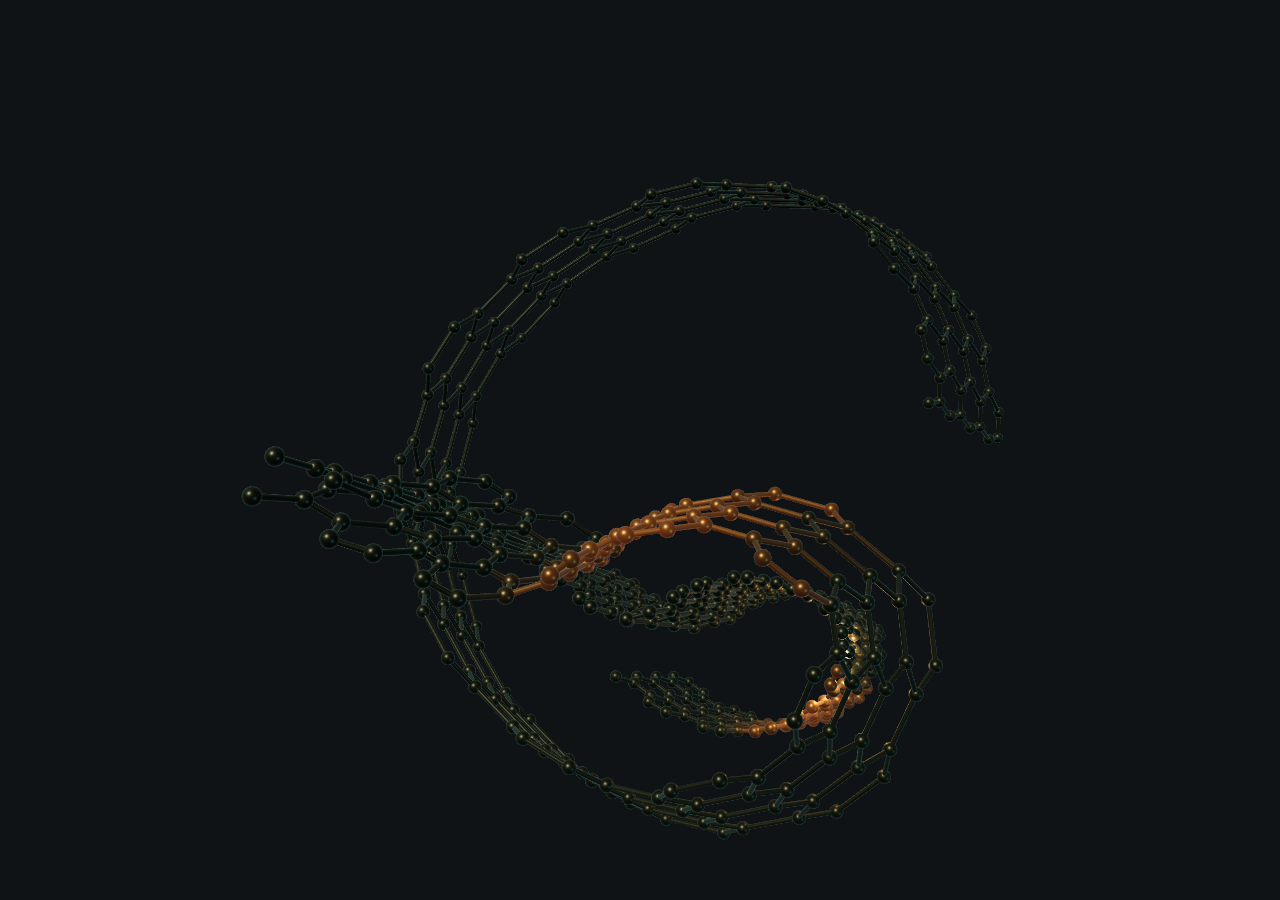
\includegraphics[width=\linewidth]{variations/renders/v1-closed.png}
  \caption{\textbf{V1 --- closed G torus.} The head and tail are joined by a
  chord across the aperture, so the loop has no free ends.}
  \label{fig:v1}
\end{subfigure}\hfill
\begin{subfigure}[b]{0.485\linewidth}
  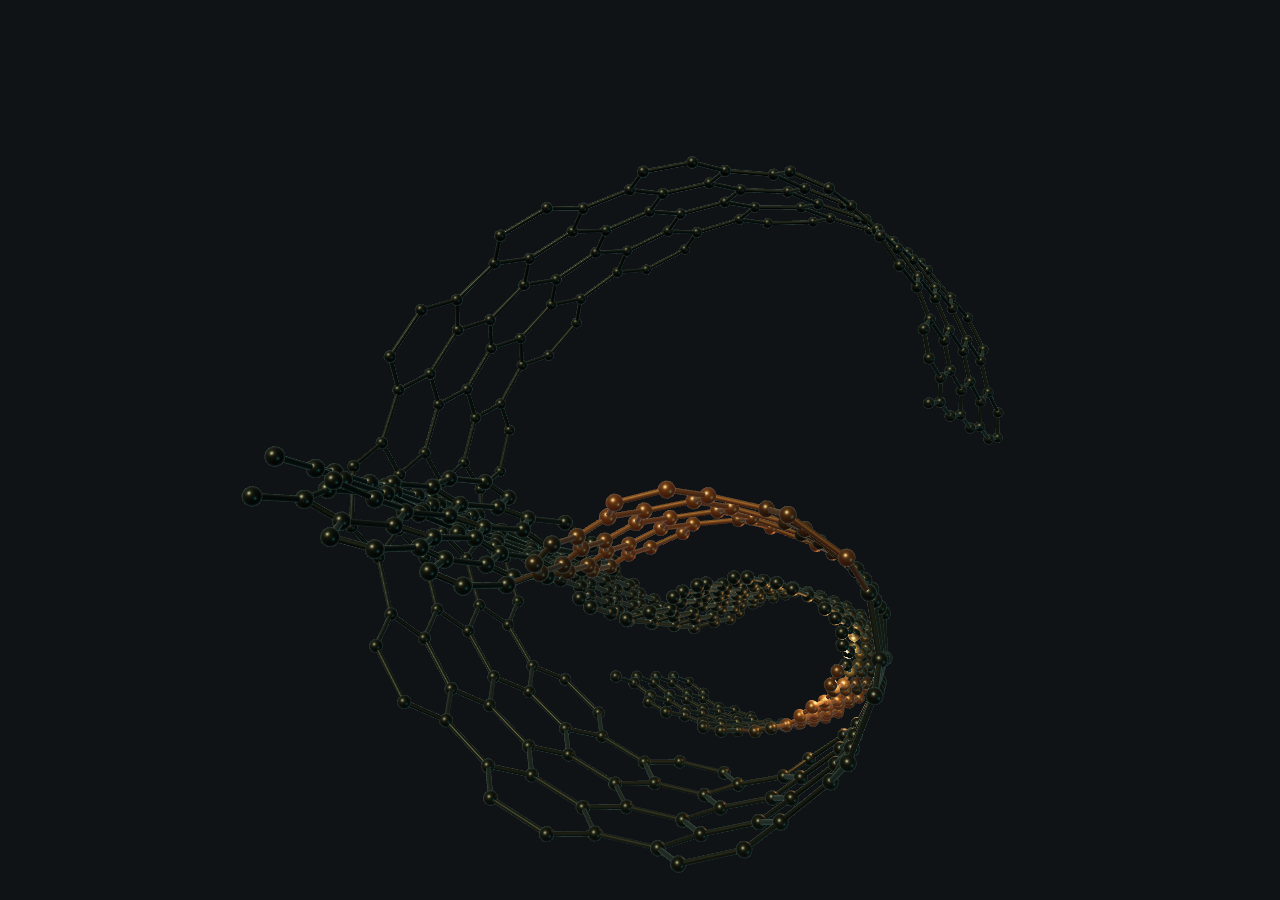
\includegraphics[width=\linewidth]{variations/renders/v2-phase-locked.png}
  \caption{\textbf{V2 --- phase-locked G torus.} The cross-section rotates
  once per lap, $k=1$, over a rotation-minimising frame.}
  \label{fig:v2}
\end{subfigure}

\vspace{6mm}
\begin{subfigure}[b]{0.485\linewidth}
  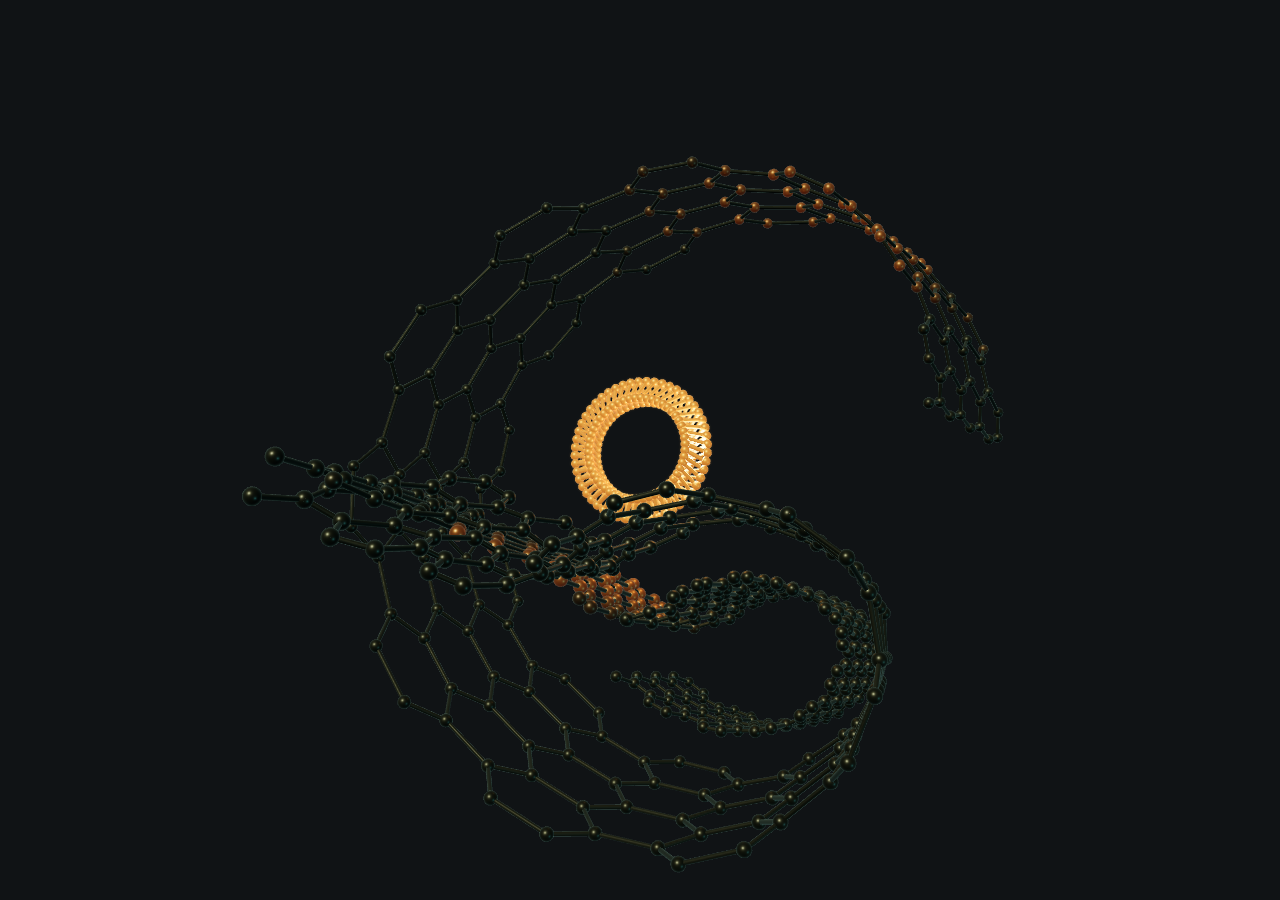
\includegraphics[width=\linewidth]{variations/renders/v3-composite.png}
  \caption{\textbf{V3 --- composite.} V2's twisted closed shell with V4's
  core on the same axis; the shell carries the period, the core the
  conjunction.}
  \label{fig:v3}
\end{subfigure}\hfill
\begin{subfigure}[b]{0.485\linewidth}
  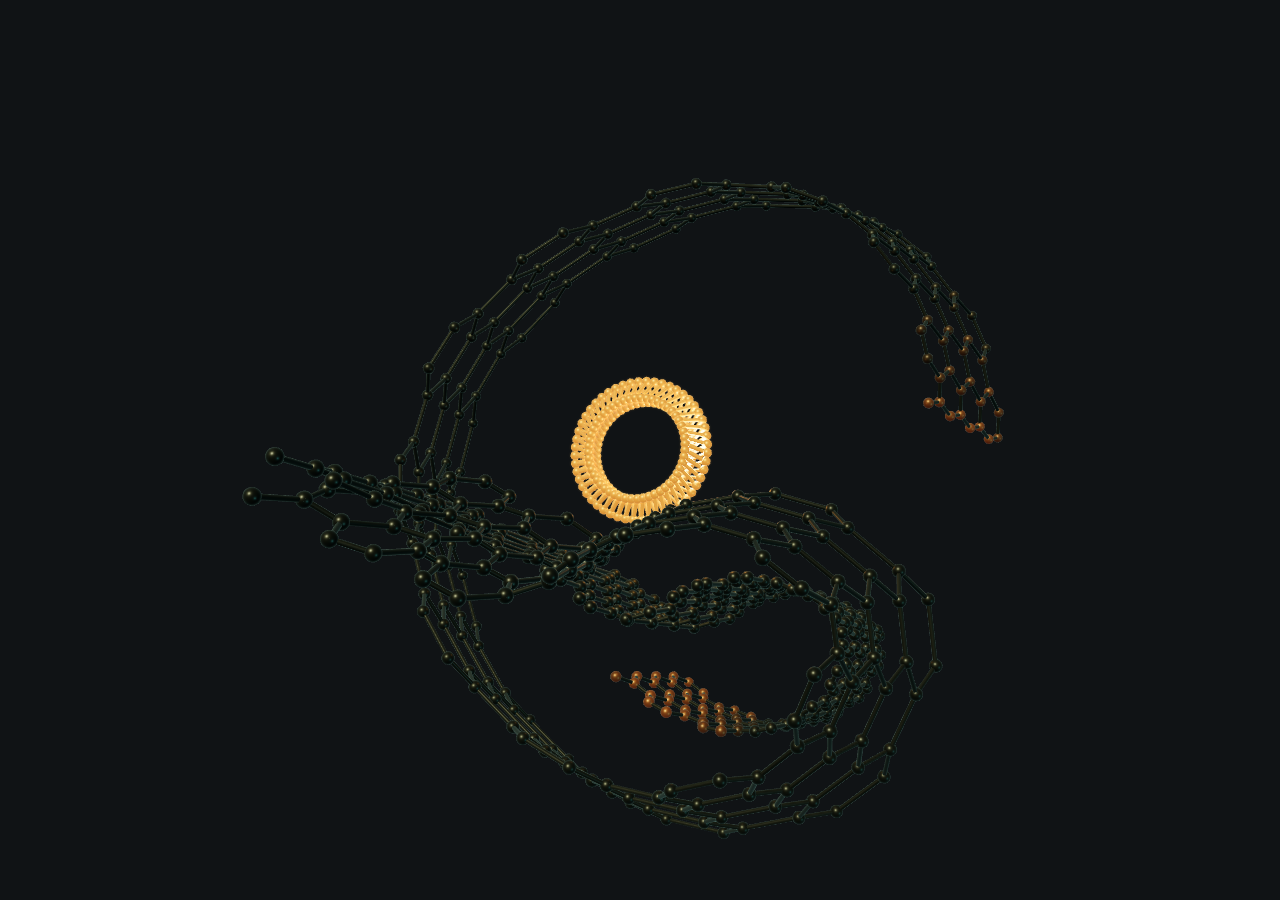
\includegraphics[width=\linewidth]{variations/renders/v4-concentric-core.png}
  \caption{\textbf{V4 --- concentric core.} A closed G shell around a small
  gold torus on the same axis.}
  \label{fig:v4}
\end{subfigure}
\caption{The four variants, rendered with the production material, lighting,
and camera. Gold marks the active signal; carbon is unlit.}
\label{fig:all}
\end{figure}

\subsection*{V1 --- closed G torus: history has no free ends}

\noindent
\textbf{Device.} Append a chord from the inner terminal to the defocused
head, resample the resulting closed polyline, and sweep the same three-row
hexagonal sheet around it with $\varphi(u)\equiv 0$:
\[
P(u,v)=\gamma(u)+r\,N(u),\qquad \gamma(0)=\gamma(1).
\]

\noindent
\textbf{Semantics.} The current shape is an open C whose two ends fade out. A
fading end is a closure violation that a viewer reads as damage rather than as
depth. Closing the loop converts the same silhouette into a solid body and, more
importantly, makes one lap \emph{mean} one period: the ring is now the domain
convention for a cyclical quantity, and position along it is the most
accurately decoded channel available. Two antipodal pulses replace the single
travelling one, because a single pulse on a closed loop has no phase reference
--- it is traffic. A pair defines the period.

\noindent
\textbf{Cost.} The chord across the aperture is not part of the logo and must be
drawn as deliberate structure. Node and bond counts are unchanged.

\subsection*{V2 --- phase-locked G torus: the period becomes geometry}

\noindent
\textbf{Device.} Keep V1's closed centreline and replace the flat frame by the
parallel-transported triple $\{T,N,B\}$, rotating the cross-section at constant
rate:
\[
\Phi_k(u,v)=\gamma(u)+r\Bigl(\cos\varphi(u)\,N(u)+\sin\varphi(u)\,B(u)\Bigr),
\qquad
\varphi(u)=\varphi_0+2\pi k u .
\]
For integer $k$ the cross-section returns to itself after one lap, so the
surface still closes with a single seam.

\noindent
\textbf{Semantics.} This is the variant the parent study recommends. The
exponential winding makes $k$ a geometric statement about the sampling period:
one lap is one period, and $k$ is the number of phase revolutions inside it. The
motif passes from edge-on to face-on around the loop, which produces an internal
light-to-dark gradient that survives at 40\,px --- exactly the legibility that
the current shape borrows from post-processing and therefore loses on mobile.
With the pulse pair running slightly off the twist rate, their beat frequency
$f_{\mathrm{beat}}=\bigl|1/T_{\mathrm{p}} - k/T_{\mathrm{t}}\bigr|$ becomes a
legible picture of two phase-locked cycles, which is the product claim rendered
as geometry.

\noindent
\textbf{Cost.} The G tail doubles back, so the transported frame can spin where
the curvature is extreme; the mitigation is to relax the tail's radius in the
control points and to clamp $\lvert d\varphi/ds\rvert r<0.6$.

\subsection*{V3 --- composite: the recommended build}

\noindent
\textbf{Device.} Superimpose the two strongest devices without blending them:
V2's helically twisted closed shell, and V4's inner torus on the same axis.
The shell keeps $k=1$ and its antipodal pulse pair; the core keeps a steady
emission at $0.38$ radius.

\noindent
\textbf{Semantics.} The two channels stay separable, which is the point. The
shell answers \emph{when}: one lap is one period, $k$ phase revolutions per
period, two pulses defining phase. The core answers \emph{what}: observations
coaxial with, and inside, relationships. Because the core is a distinct body
rather than a texture on the shell, the eye reads a two-part object, and the
sentence \emph{relationships and observations, together} becomes a statement
about containment instead of a caption. The twist supplies an internal
light-to-dark gradient, so the reading survives at small sizes and without
post-processing.

\noindent
\textbf{Cost.} Two assemblies in one draw path, and the core must stay inside
the aperture at every rotation. In practice this is the cheapest version of the
recommended design, because it reuses the two previous parameterisations
unchanged.

\subsection*{A rejected variant, and why}

\noindent
An earlier fifth candidate, a \emph{temporal stack} --- five contours of the
same G at increasing depth joined by rungs, one contour lit --- is archived in
\texttt{variations/archive/} rather than presented. Its semantics were the most
literal of all: a layer is a snapshot, rungs are state transitions, depth is
time. It was rejected on visual grounds, not semantic ones. Five superimposed
contours destroy the silhouette, the rungs read as a grid rather than as
causality, and the object no longer holds together as a body --- which
contradicts the one rule the rest of the set obeys. Recording the rejection
matters: the failure is informative, because it shows that encoding time
\emph{as layers} competes with encoding time \emph{as position}, and only one
of them can own the silhouette.

\subsection*{V4 --- concentric core: two data models, one axis}

\noindent
\textbf{Device.} Keep V1's closed shell at radius $\sim2$ and add a small torus
of radius $0.38$ on the same axis, sharing the same material but permanently
emissive, with the shell carrying the travelling pulse.

\noindent
\textbf{Semantics.} This is the most literal reading of the positioning
sentence. The outer lattice is relationships; the inner ring is observations;
they are concentric and coaxial, so neither is privileged and the claim
\emph{relationships and observations, together} is a geometric fact rather than
a caption. It also produces the strongest depth cue in the set --- a genuinely
occluded core --- which is what makes the object read as photographed.

\noindent
\textbf{Cost.} A second primitive assembly in one draw path, and the core must be
small enough to stay inside the aperture at every rotation.

\section{Comparison}

\begin{table}[htbp]
\centering
\small
\begin{tabular}{@{}p{0.16\linewidth}p{0.22\linewidth}p{0.24\linewidth}p{0.26\linewidth}@{}}
\toprule
\textbf{Variant} & \textbf{Geometric device} & \textbf{Semantic channel} & \textbf{Cost} \\
\midrule
V1 closed G torus &
close the loop, $\varphi=0$ &
one lap $=$ one period; no dissolved ends &
chord across the aperture must read as designed \\
\addlinespace
V2 phase-locked &
helical sweep, $k=1$, transported frame &
period and phase as geometry; beat frequency &
frame spin at the doubled-back tail \\
\addlinespace
V3 composite &
twisted closed shell $+$ inner core &
shell carries the period, core the conjunction &
two assemblies in one draw path \\
\addlinespace
V4 concentric core &
closed shell $+$ inner torus &
relations outside, observations inside, coaxial &
second assembly; core must fit the aperture \\
\bottomrule
\end{tabular}
\caption{Each variant buys one clear channel and pays in exactly one place.
V2 is the recommendation of the parent study; V4 is the strongest purely visual
option; V1 is the cheapest and safest; V3 is the most literal about the data.}
\label{tab:compare}
\end{table}

\section{Reproduction}

\begin{verbatim}
cd site
npm run dev
PREVIEW_BASE=http://127.0.0.1:5174/graphfin \
PLAYWRIGHT_CHROMIUM_EXECUTABLE=... \
  node research/variations/capture.mjs
pdflatex hero-g-variations.tex
\end{verbatim}

\noindent
\texttt{research/variations/preview.js} builds each variant from the same logo
skeleton used by the production hero, so the silhouette cannot drift from the
brand mark. \texttt{?v=} selects a variant and \texttt{?z=} overrides the camera
distance. The rejected temporal stack is retained in
\texttt{variations/archive/} and is still reachable with \texttt{?v=stack}.

\end{document}
